\documentclass[a4paper,11pt]{article}

%%%%%%%%%%%%%%%%%%%%%%%%%%%%%%%%%%%%%%%%%%%%% General %%%%%%%%%%%%%%%%%%%%%%%%%%%%%%%%%%%%%%%%%%%%%%
\usepackage[dvipsnames]{xcolor}
\usepackage{nameref}
\usepackage{acronym}
\usepackage{enumitem}
\usepackage{multirow}


%%%%%%%%%%%%%%%%%%%%%%%%%%%%%%%%%%%%%%%%%% Mise en page %%%%%%%%%%%%%%%%%%%%%%%%%%%%%%%%%%%%%%%%%%%%
\usepackage[left=2cm,right=2cm,top=3cm,bottom=3.2cm]{geometry}
\usepackage[T1]{fontenc}
\usepackage[english]{babel}
\usepackage[latin1]{inputenc}

%%%%%%%%%%%%%%%%%%%%%%%%%%%%%%%%%%%%%%%%%%% Références %%%%%%%%%%%%%%%%%%%%%%%%%%%%%%%%%%%%%%%%%%%%%
\usepackage[colorlinks=true,linkcolor=black,filecolor=magenta,urlcolor=black,citecolor=blue]{hyperref}  

%%%%%%%%%%%%%%%%%%%%%%%%%%%%%%%%%%%%%%%%%%%%%% Maths %%%%%%%%%%%%%%%%%%%%%%%%%%%%%%%%%%%%%%%%%%%%%%%
\usepackage{bm}
\usepackage{amsthm}
\usepackage{amsmath}
\usepackage{amssymb}
\usepackage[cmintegrals]{newtxmath}

%%%%%%%%%%%%%%%%%%%%%%%%%%%%%%%%%%%%%%%%%%%%%% TIK'Z %%%%%%%%%%%%%%%%%%%%%%%%%%%%%%%%%%%%%%%%%%%%%%%
\usepackage{tikz,tkz-tab}
\usetikzlibrary{calc}
\usepackage{pgfplots}
\pgfplotsset{compat=1.3}

%%%%%%%%%%%%%%%%%%%%%%%%%%%%%%%%%%%%%%%%%%% Algorithmic %%%%%%%%%%%%%%%%%%%%%%%%%%%%%%%%%%%%%%%%%%%%
\usepackage{algorithm}
\usepackage{algorithmicx}
\usepackage[noend]{algpseudocode}

%%%%%%%%%%%%%%%%%%%%%%%%%%%%%%%%%%%%%%%%%%%%% Graphics %%%%%%%%%%%%%%%%%%%%%%%%%%%%%%%%%%%%%%%%%%%%%
\usepackage{url}
\usepackage{subfig}
\usepackage{wrapfig}
\usepackage{graphicx}
\usepackage{pgfplots}
\usepackage{subfloat}
\usepackage{epstopdf}

%%%%%%%%%%%%%%%%%%%%%%%%%%%%%%%%%%%%%%%%%%%%% Commands %%%%%%%%%%%%%%%%%%%%%%%%%%%%%%%%%%%%%%%%%%%%%
\newcommand{\Z}{\mathbb{Z}}
\newcommand{\Q}{\mathbb{Q}}
\newcommand{\F}{\mathbb{F}}
\newcommand{\R}{\mathcal{R}}
\newcommand{\K}{\mathcal{K}}
\renewcommand{\S}{\mathcal{S}}
\newcommand{\rand}{\xleftarrow{\$}}
\newcommand{\todo}{\textcolor{red}{TODO }}
\newcommand{\prodscal}[2]{\left\langle#1, #2\right\rangle}

%%%%%%%%%%%%%%%%%%%%%%%%%%%%%%%%%%%%%%%%%% Math Operators %%%%%%%%%%%%%%%%%%%%%%%%%%%%%%%%%%%%%%%%%%
\DeclareMathOperator{\Gal}{Gal}

%%%%%%%%%%%%%%%%%%%%%%%%%%%%%%%%%%%%%%%%%%%%% Theorems %%%%%%%%%%%%%%%%%%%%%%%%%%%%%%%%%%%%%%%%%%%%%
\theoremstyle{definition}
\newtheorem{theorem}{\bf{Theorem}}[section]
\newtheorem{lemma}[theorem]{\bf{Lemma}}
\newtheorem{remark}[theorem]{\bf{Remark}}
\newtheorem{example}[theorem]{\bf{Example}}
\newtheorem{corollary}[theorem]{\bf{Corollary}}
\newtheorem{definition}[theorem]{\bf{Definition}}
\newtheorem{proposition}[theorem]{\bf{Proposition}}

%%%%%%%%%%%%%%%%%%%%%%%%%%%%%%%%%%%%%%%%%%%%% Acro-Def %%%%%%%%%%%%%%%%%%%%%%%%%%%%%%%%%%%%%%%%%%%%%
\acrodef{GC}{Garbled Circuit}
\acrodef{FV}{Fan-Vercauteren}
\acrodef{SP}{Streaming Processor}
\acrodef{GSW}{Gentry-Sahai-Waters}
\acrodef{HAO}{Hiromasa-Abe-Okamoto}
\acrodef{LWE}{Learning With Errors}
\acrodef{HE}{Homomorphic Encryption}
\acrodef{LSB}{Least Significant Bit}
\acrodef{ANF}{Algebraic Normal Form}
\acrodef{RNS}{Residue Number System}
\acrodef{SVM}{Support Vector Machine}
\acrodef{SVP}{Shortest Vector Problem}
\acrodef{CPU}{Central Processing Unit}
\acrodef{GPU}{Graphics Processor Unit}
\acrodef{CRT}{Chinese Remainder Theorem}
\acrodef{SMP}{Symmetric Multiprocessing}
\acrodef{LLL}{Lenstra Lenstra Lov{\'a}sz}
\acrodef{NTT}{Number Theoretic Transform}
\acrodef{DFT}{Discrete Fourier Transform}
\acrodef{HPC}{High Performance Computing}
\acrodef{APU}{Accelerated Processing Unit}
\acrodef{LTV}{Lopez-Tromer-Vaikuntanathan}
\acrodef{FHE}{Fully Homomorphic Encryption}
\acrodef{GMDH}{Group Method of Data Handling}
\acrodef{Ring-LWE}{Ring-Learning With Errors}
\acrodef{FPGA}{Field-Programmable Gate Array}
\acrodef{SHE}{Somewhat Homomorphic Encryption}
\acrodef{BGV}{Brakerski-Gentry-Vaikuntanathan}
\acrodef{SIMD}{Single Instruction Multiple Data}
\acrodef{DSPR}{Decisional Small Polynomial Ratio}
\acrodef{SIVP}{Shortest Independent Vectors Problem}
\acrodef{S(I)VP}{Shortest (Independent) Vector Problem}
\acrodef{YASHE'}{Yet Another Somewhat Homomorphic Encryption'}

%%%%%%%%%%%%%%%%%%%%%%%%%%%%%%%%%%%%%%%%%%%%%%%%%%%%%%%%%%%%%%%%%%%%%%%%%%%%%%%%%%%%%%%%%%%%%%%%%%%%

\title{Comparison circuit over $\mathbb{F}_{p^d}$}
\date{}
\author{}

\begin{document}
\maketitle

We want to compare two vectors $X=(x_1,x_2,\ldots,x_\ell)$ and $Y=(y_1,y_2,\ldots,y_\ell)\in\mathbb{F}_{p^d}^\ell$ for the lexicographical order $<_L$:

$$X <_L Y \Leftrightarrow \exists i\in[1,\ell] \text{ such that } x_i < y_i \text{ and } \forall j\leq i ~~ x_j = y_j $$

where $x<y$ compare $x$ and $y$ as if they were elements of $[0,p^d-1]$. Let us assume that we can compute the logical gates $<$ and $=$ over $\mathbb{F}_{p^d}$, then we can evaluate the lexicographical order $<_L$ as: 

$$ X <_L Y = \sum_{i=1}^\ell \left( (x_i < y_i).\prod_{j=1}^{i-1} (x_i = y_j) \right)$$

We can evaluate the term $\prod_{j=1}^{i-1} (x_i = y_j)$ using the randomized vector equality testing with a depth independant of $i$. We are left with evaluating $<$ over $\mathbb{F}_q$ for $q=p^d$ whose truth table is given hereafter:

$$
\begin{array}{c|ccccc}
  < & 0 & 1 & 2 & \cdots & q-1 \\
  \hline
  0 & 0 & 1 & 1 & \cdots & 1 \\
  1 & 0 & 0 & 1 & \cdots & 1 \\
  2 & 0 & 0 & 0 & \cdots & 1 \\
  \vdots & \vdots & \vdots & \vdots & \ddots & \vdots \\
  q-1 & 0 & 0 & 0 & \cdots & 0 \\
\end{array}
$$

Therefore it can be evaluated as:

\begin{align*}
  x < y & = \sum_{i=0}^{q-2} \left( (x = i)\cdot \prod_{j=0}^i (y \neq j) \right) \\
        & = \sum_{i=0}^{q-2} \left( (x = i)\cdot \sum_{j=i+1}^{q-1} (y = j) \right) \\
\end{align*}

We denote the function $f: \mathbb{F}_q \rightarrow \mathbb{F}_q$ defined by $f(x) = x^{q-1}$ which is equal to $0$ if $x = 0$ and $1$ otherwise, thus we have $(x = j) = 1-f(x-j)$. As a consequence we can write $<$ as:

$$ x < y = \sum_{i=0}^{q-2} \left( (1-f(x-i)) \cdot \sum_{j=i+1}^{q-1} (1 - f(y-j)) \right) $$

Suppose we have two ciphertexts encrypting the vectors of length $q-1$ (can be of length $k\geq q-1$ with $0$s padding) $(x,0,\ldots,0)$ and $(y,0,\ldots,0)$ in an SIMD fashion. We can obtain ciphertexts encrypting $(x,x,\ldots, x)$ and $(y,y,\ldots, y)$ with $2\log_2(q-1)\texttt{Rot}$ and $2\log_2(q-1)\texttt{Add}$. 

From there we can obtain encryptions of $(x,x-1,\ldots, x-q-2)$ and $(y-1,y-2,\ldots, y-q-1)$ with $2\texttt{Add}$. We can apply $f$ to these vectors in parallel with a depth of $\log (p-1) + \log d$ for a cost of $2(\log (p-1) + wt(p-1) + d - 2) \texttt{Mult}$. This can be minimized by choosing $p = 2^d + 1$ for some $d$.

With $2$ more $\texttt{Sub}$ we obtain encryptions of $(1-f(x), 1-f(x-1), \ldots, 1-f(x-q-2))$ and $(1-f(y-1), 1-f(y-2), \ldots, 1-f(y-q-1))$. From there we can get an ecryption of the different partial sums in $\log_2(q-1)\texttt{Rot}$, $\log_2(q-1)\texttt{Select}$ and $\log_2(q-1)\texttt{Add}$. The algorithm works as follow:

\begin{center}
  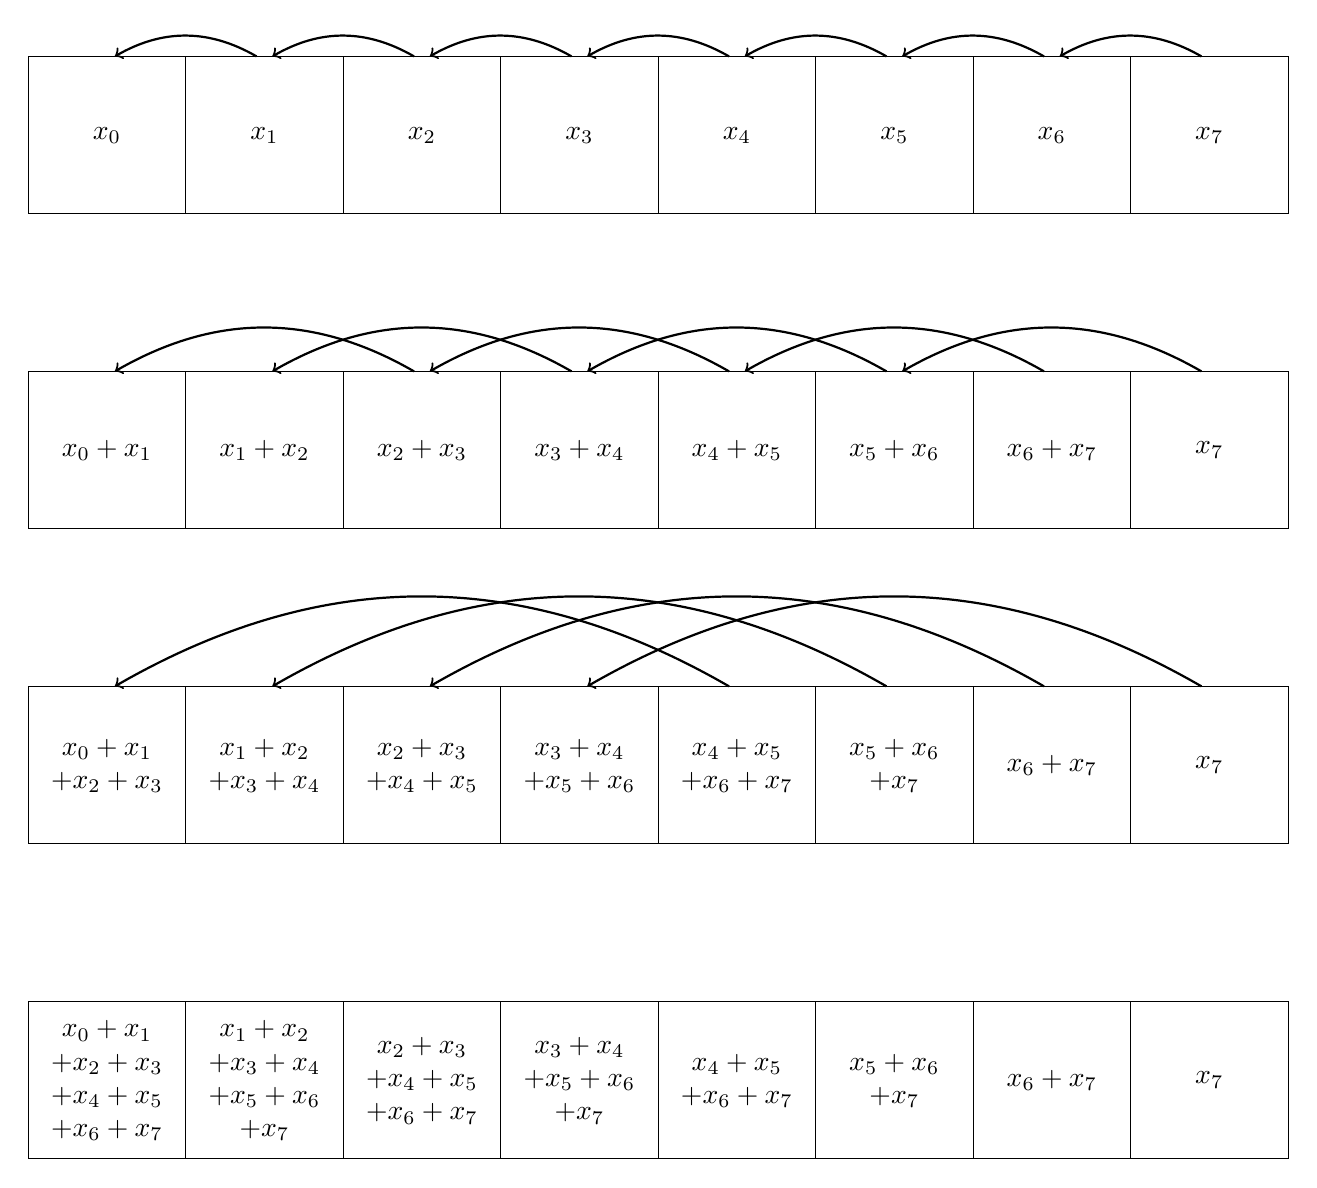
\begin{tikzpicture}
    \newcommand\y{-4};
    
    \draw (0,2) -- (16,2);
    \draw (0,0) -- (16,0);    
    \foreach \x in {0,...,8}{
      \draw (2*\x,0) -- (2*\x,2);
    }
    \foreach \x in {0,...,7}{
      \node at (2*\x+1,1) {$x_\x$};
    }

    \draw (0,2+\y) -- (16,2+\y);
    \draw (0,\y) -- (16,\y);    
    \foreach \x in {0,...,8}{
      \draw (2*\x,0+\y) -- (2*\x,2+\y);
    }

    \node at (1,1+\y) {$x_0 + x_1$};
    \node at (3,1+\y) {$x_1 + x_2$};
    \node at (5,1+\y) {$x_2 + x_3$};
    \node at (7,1+\y) {$x_3 + x_4$};
    \node at (9,1+\y) {$x_4 + x_5$};
    \node at (11,1+\y) {$x_5 + x_6$};
    \node at (13,1+\y) {$x_6 + x_7$};
    \node at (15,1+\y) {$x_7$};

    %%%%%%%%%%%%%%%%%%%%%%%%%%%%%%%%%%%%
    
    \draw (0,2+2*\y) -- (16,2+2*\y);
    \draw (0,0+2*\y) -- (16,0+2*\y);    
    \foreach \x in {0,...,8}{
      \draw (2*\x,0+2*\y) -- (2*\x,2+2*\y);
    }

    \node at (1,1+2*\y) {$\begin{array}{c}
        x_0 + x_1  \\
        + x_2 + x_3
      \end{array}$};
    \node at (3,1+2*\y) {$\begin{array}{c}
        x_1 + x_2  \\
        + x_3 + x_4
      \end{array}$};
    \node at (5,1+2*\y) {$\begin{array}{c}
        x_2 + x_3  \\
        + x_4 + x_5
      \end{array}$};
    \node at (7,1+2*\y) {$\begin{array}{c}
        x_3 + x_4  \\
        + x_5 + x_6
      \end{array}$};
    \node at (9,1+2*\y) {$\begin{array}{c}
        x_4 + x_5  \\
        +x_6 + x_7
      \end{array}$};
    \node at (11,1+2*\y) {$\begin{array}{c}
        x_5 + x_6  \\
        + x_7
      \end{array}$};
    \node at (13,1+2*\y) {$x_6 + x_7$};
    \node at (15,1+2*\y) {$x_7$};

    %%%%%%%%%%%%%%%%%%%%%%%%%%%%%%%%%%%%%%%%%%
    
    \draw (0,2+3*\y) -- (16,2+3*\y);
    \draw (0,0+3*\y) -- (16,0+3*\y);    
    \foreach \x in {0,...,8}{
      \draw (2*\x,0+3*\y) -- (2*\x,2+3*\y);
    }

    \node at (1,1+3*\y) {$\begin{array}{c}
        x_0 + x_1  \\
                            + x_2 + x_3 \\
                            + x_4 + x_5 \\
                            + x_6 + x_7
      \end{array}$};
    \node at (3,1+3*\y) {$\begin{array}{c}
        x_1 + x_2  \\
                            + x_3 + x_4 \\
                            + x_5 + x_6 \\
                            + x_7 \\
      \end{array}$};
    \node at (5,1+3*\y) {$\begin{array}{c}
        x_2 + x_3  \\
                            + x_4 + x_5 \\
                            + x_6 + x_7
      \end{array}$};
    \node at (7,1+3*\y) {$\begin{array}{c}
        x_3 + x_4  \\
                            + x_5 + x_6 \\
                            +x_7
      \end{array}$};
    \node at (9,1+3*\y) {$\begin{array}{c}
        x_4 + x_5  \\
        +x_6 + x_7
      \end{array}$};
    \node at (11,1+3*\y) {$\begin{array}{c}
        x_5 + x_6  \\
        + x_7
      \end{array}$};
    \node at (13,1+3*\y) {$x_6 + x_7$};
    \node at (15,1+3*\y) {$x_7$};

    \foreach \x in {2,...,8}
    \draw[->,thick = 2pt] (2*\x-0.1-1,2) to[bend right] (2*\x-3+0.1,2);

    \foreach \x in {3,...,8}
    \draw[->,thick = 2pt] (2*\x-0.1-1,2+\y) to[bend right] (2*\x-5+0.1,2+\y);

    \foreach \x in {5,...,8}
    \draw[->,thick = 2pt] (2*\x-0.1-1,2+2*\y) to[bend right] (2*\x-9+0.1,2+2*\y);

\end{tikzpicture}
\end{center}

From there we just have to compute the scalar product of the two vectors with $1\texttt{Mult} + \log_2(q-1)\texttt{Rot} + \log_2(q-1)\texttt{Add}$. \newline

So overall we can compute $<$ over $\mathbb{F_q}$ for $q = p^d$ in:

\begin{itemize}
\item $4\log_2 (q-1) \texttt{Rot}$
\item $(4\log_2 (q-1) + 4) \texttt{Add}$
\item $(2(\log (p-1) + wt(p-1) + d - 2) + 1) \texttt{Mult}$
\item $(\log_2 (q-1) + 1) \texttt{Select}$
\end{itemize}

\end{document}

%%% Local Variables:
%%% mode: latex
%%% TeX-master: t
%%% End:
